\begin{figure}[h!]
  \centering
  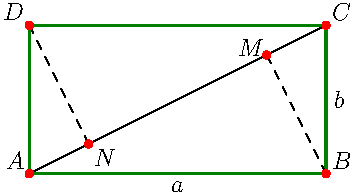
\includegraphics{Egp13_1.pdf}
  \caption{Exercice \arabic{enumi}}
  \label{fig:Egp13_1}
\end{figure}

\begin{tiny}(gp13)\end{tiny} Soit $A$, $B$, $C$, $D$  un rectangle dont les longueurs des côtés sont $a$ et $b$. On projette les points $B$ et $D$ en $M$ et $N$ sur la diagonale $(AC)$. (voir figure \ref{fig:Egp13_1}).\newline
Exprimer la longueur $MN$ en fonction de $a$ et $b$.
